\documentclass[12pt, oneside]{article} 
\usepackage[left=15mm, right=15mm, top=10mm]{geometry}
\usepackage{graphicx}
\usepackage{url}
\usepackage{multicol}
\usepackage{lipsum}
\usepackage{mwe}
\usepackage{float}

\begin{document}
\title{Techniques d'attaque - injection de traffic}
\author{Tristan BILOT, Nora DELFAU, Enzar SALEMI, Madushan THAMBITHURAI\\EPITA}
\date{7 Juin 2021}
\maketitle

\begin{abstract}
L'objectif de ce TP est d'utiliser est de manipuler les requêtes de niveau 3 et les trames de niveau afin de mettre en places des attaques de type Man in the middle ou DNS poisoning. Les outils utilisés sont wireshark, ettercap, arpspoof et scapy. Une implémentation détaillée développée à l'aide de scapy est disponible à la fin de ce document.
\end{abstract}

\section{Notes}
\subsection{Man in the middle}
Man in the middle: l'objectif est de se mettre en tant que proxy entre le serveur et l'utilisateur cible.
\subsection{ARP}
ARP est le protocole permettant de mapper les adresses IP d'un réseau avec leur adresse MAC. Au moment d'en envoi d'une requête à une adresse IP, à la couche de session, la table ARP va d'abord être consultée afin de trouver la MAC associée à l'adresse IP. Dans le cas où l'adresse IP n'est pas dans la table, un broadcast est lancé afin de demander l'adresse MAC.
L'adresse MAC d'une machine peut être modifiée au niveau logiciel. Le routage d'un réseau à un autre réseau se fait au niveau 3. Au niveau 2, une trame sera envoyée à la gateway qui elle transmettra le message au deuxième réseau.
\begin{itemize}
\item Man in the  middle: on se fait passer pour la gateway, donc on envoie notre adresse MAC à la place de celle de la gateway. cela permet de récupérer les requêtes envoyées initialement à la gateway. La machine victime de l'attaque va rentrer l'adresse MAC de l'attaquant dans sa table ARP et échangera désormais avec lui.
\item DNS poisoning: en se mettant à la place du dns, on associe à des noms de domaine les mauvaises adresses IP. Ainsi, il est possible de rediriger l'accès à google.com vers un autre site Internet.
\item Deux outils connus pour les attaques man in the middle: Aprspoof, Ettercap. Si un site est requeté et qu'on se positionne entre les le serveur et la machine ciblée, il est possible de modifier le contenu du site Internet si TLS n'est pas utilisé. Sinon, il ne sera pas possible de modifier le site vu que la réponse sera chiffrée.
\item Dans les outils de scan comme nmap, des paquets SYN sont envoyés sur les ports, c'est ensuit en fonction de la réponse que des décisions seront prises: si la réponse est un SYN ACK, c'est que le port est ouvert, s'il n'y a pas de réponse, c'est que le port est fermé, sinon si un paquet ICMP est retournée c'est un firewall qui a bloqué la connexion.
\end{itemize}

\section{Exercice 1}
Dans les prochaines étapes, chaque envoi de requête sera examinée grâce à wireshark afin de comprendre en détail le fonctionnement derrière chaque requête.
Il est possible d'envoyer une trame ethernet grâce à la commande sendp (Fig 1). Il faudra spécifier l'adresse MAC de destination, l'IP ainsi que le protocole à utiliser.\\
On lance le service apache sur la machine distante grâce à cette commande:
\begin{figure}[H]
\centering
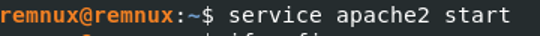
\includegraphics[scale=0.7]{1}
\caption{lancement d'un serveur Apache}
\end{figure}
Nous avons créé un script pour pouvoir effectuer les commandes plus simplement, dans ce script nous définissons les deux IP importantes:
\begin{itemize}
\item l’IP source qui correspond à notre machine
\item l’IP destination qui correspond à la machine que l’on va attaquer
\end{itemize}
On envoie un paquet  comportant la requête SYN et on randomise le numéro de port(entre 420 et 600)  à chaque envoi et on établit comme port source : le 18
\begin{figure}[H]
\centering
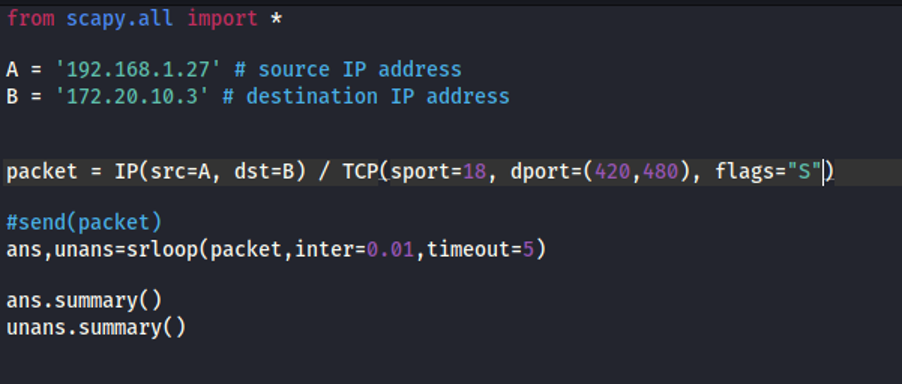
\includegraphics[scale=0.7]{2}
\end{figure}
Ensuite en commentaire nous avons la fonction send() qui va envoyer le paquet.
On lance l’attaque avec la fonction srloop() avec un intervalle entre chaque envoie de 0.01 secondes et le timeout réglé à 5 secondes
\begin{figure}[H]
\centering
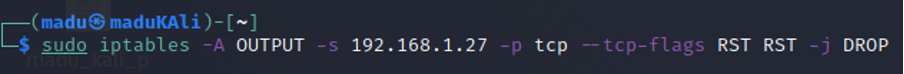
\includegraphics[scale=0.7]{3}
\end{figure}
Afin d’éviter d’envoyer des RST au noyau de la machine distante, on ajoute une règle pour palier à ce problème.
\begin{figure}[H]
\centering
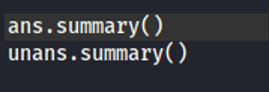
\includegraphics[scale=0.7]{4}
\end{figure}
On va donc afficher les résultats de notre attaque avec ans(celles qui ont été répondu et celles qui ne l’ont pas été)
\begin{figure}[H]
\centering
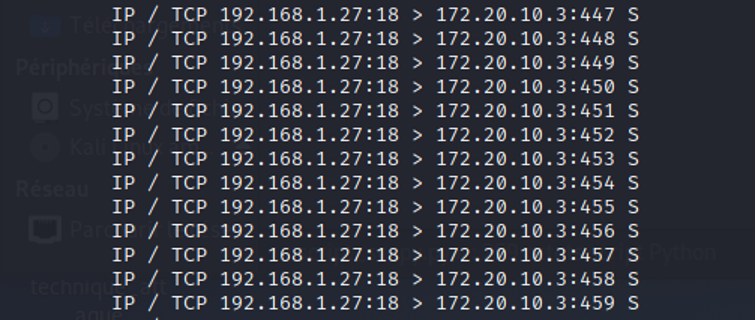
\includegraphics[scale=0.7]{5}
\end{figure}
L’envoi du paquet avec srloop et on peut voir l’affichage de tous les paquets envoyés à chaque port.
\begin{figure}[H]
\centering
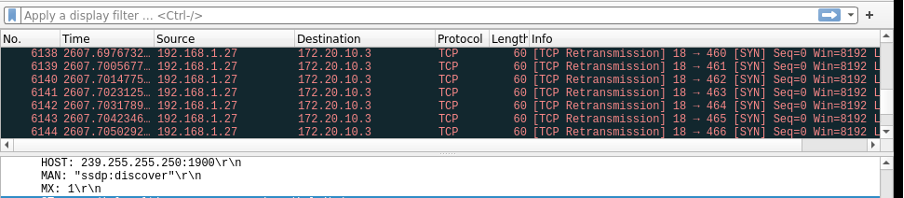
\includegraphics[scale=0.7]{6}
\end{figure}
Les résultats de l’attaque sont affiché sur le Wireshark de la machine distante.
\begin{figure}[H]
\centering
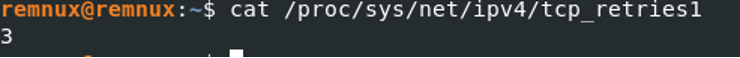
\includegraphics[scale=0.7]{7}
\end{figure}
Grâce à cette commande, nous avons le temps d’attente du système après la réception d’un SYN.


\section{Exercice 2}
Port 80 : SYN :
\begin{figure}[H]
\centering
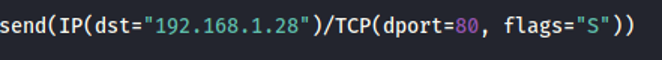
\includegraphics[scale=0.7]{8}
\end{figure}
\begin{itemize}
\item port ouvert :  On obtient la réponse SYN/ACK
\begin{figure}[H]
\centering
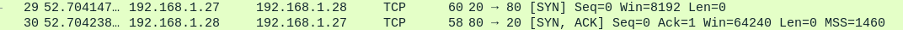
\includegraphics[scale=0.7]{9}
\end{figure}
\item port fermé: On obtient la réponse RST/ACK
\begin{figure}[H]
\centering
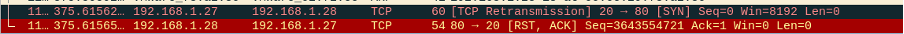
\includegraphics[scale=0.7]{10}
\end{figure}
\end{itemize}

Port 80 : Push, Fin, Urgent avec la commande :
\begin{figure}[H]
\centering
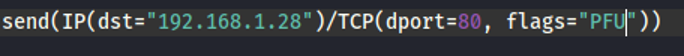
\includegraphics[scale=0.7]{11}
\end{figure}
\begin{itemize}
\item port ouvert: Nous n’obtenons pas de réponse
\begin{figure}[H]
\centering
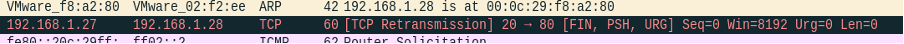
\includegraphics[scale=0.7]{12}
\end{figure}
\item port fermé: On reçoit la réponse RST/ACK
\begin{figure}[H]
\centering
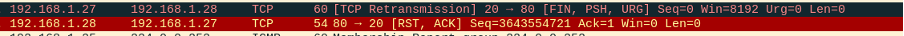
\includegraphics[scale=0.7]{13}
\end{figure}
\end{itemize}

Port 80: FIN avec la commande:
\begin{figure}[H]
\centering
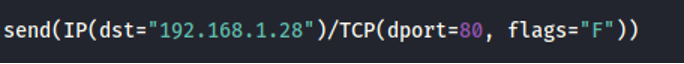
\includegraphics[scale=0.7]{14}
\end{figure}
\begin{itemize}
\item port ouvert: Nous n’obtenons pas de réponse
\begin{figure}[H]
\centering
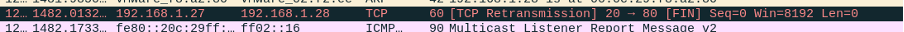
\includegraphics[scale=0.7]{15}
\end{figure}
\item port fermé: On reçoit la réponse RST/ACK
\begin{figure}[H]
\centering
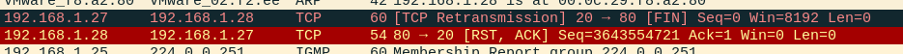
\includegraphics[scale=0.7]{16}
\end{figure}
\end{itemize}

Port 80 : Sans flags avec la commande : 
\begin{figure}[H]
\centering
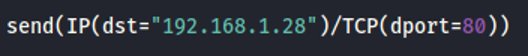
\includegraphics[scale=0.7]{17}
\end{figure}
\begin{itemize}
\item port ouvert: Nous obtenons la réponse SYN/ACK
\begin{figure}[H]
\centering
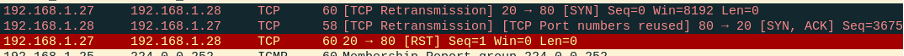
\includegraphics[scale=0.7]{18}
\end{figure}
\item port fermé: Nous obtenons la réponse RST/ACK
\begin{figure}[H]
\centering
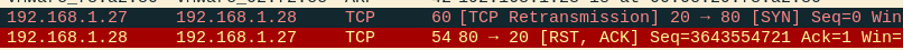
\includegraphics[scale=0.7]{19}
\end{figure}
\end{itemize}


\subsection{IP source spoofing}
\begin{figure}[H]
\centering
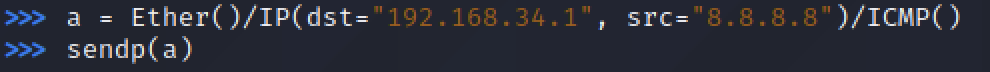
\includegraphics[scale=0.4]{sendp2}
\caption{Trame ethernet envoyée avec une source 8.8.8.8 modifiée}
\end{figure}
Comme prévu, la source est bien modifiée sur wireshark.
\begin{figure}[H]
\centering
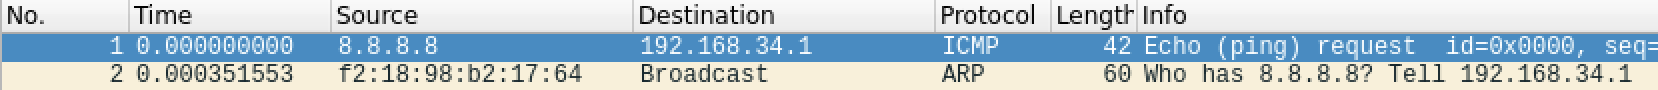
\includegraphics[scale=0.4]{wire2}
\caption{Trame ethernet provenant de 8.8.8.8}
\end{figure}

\subsection{Envoie de paquets à des ports aléatoires}
Il est possible d'envoyer des paquets sur des ports aléatoires en utilisant RandShort(). Côté wireshark, on constate que toutes les requêtes échouent étant donné que les numéros de ports sont fermés, il n'y a donc pas de réponse de la machine scannée. 
\begin{figure}[H]
\centering
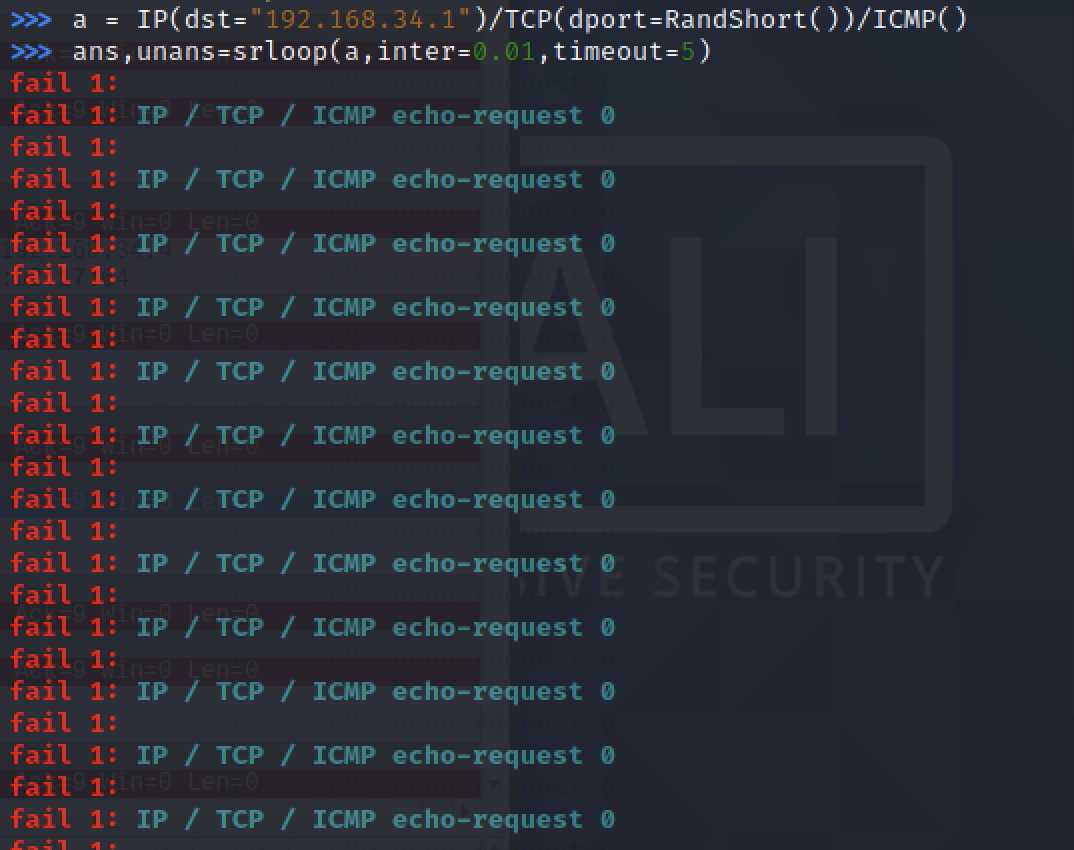
\includegraphics[scale=0.4]{sendp3}
\caption{Envoi de paquets en boucle à des ports aléatoires}
\end{figure}
En examinant chaque paquet, on voit bien que le port est à chaque fois différent (28432, 28178...).
\begin{figure}[H]
\centering
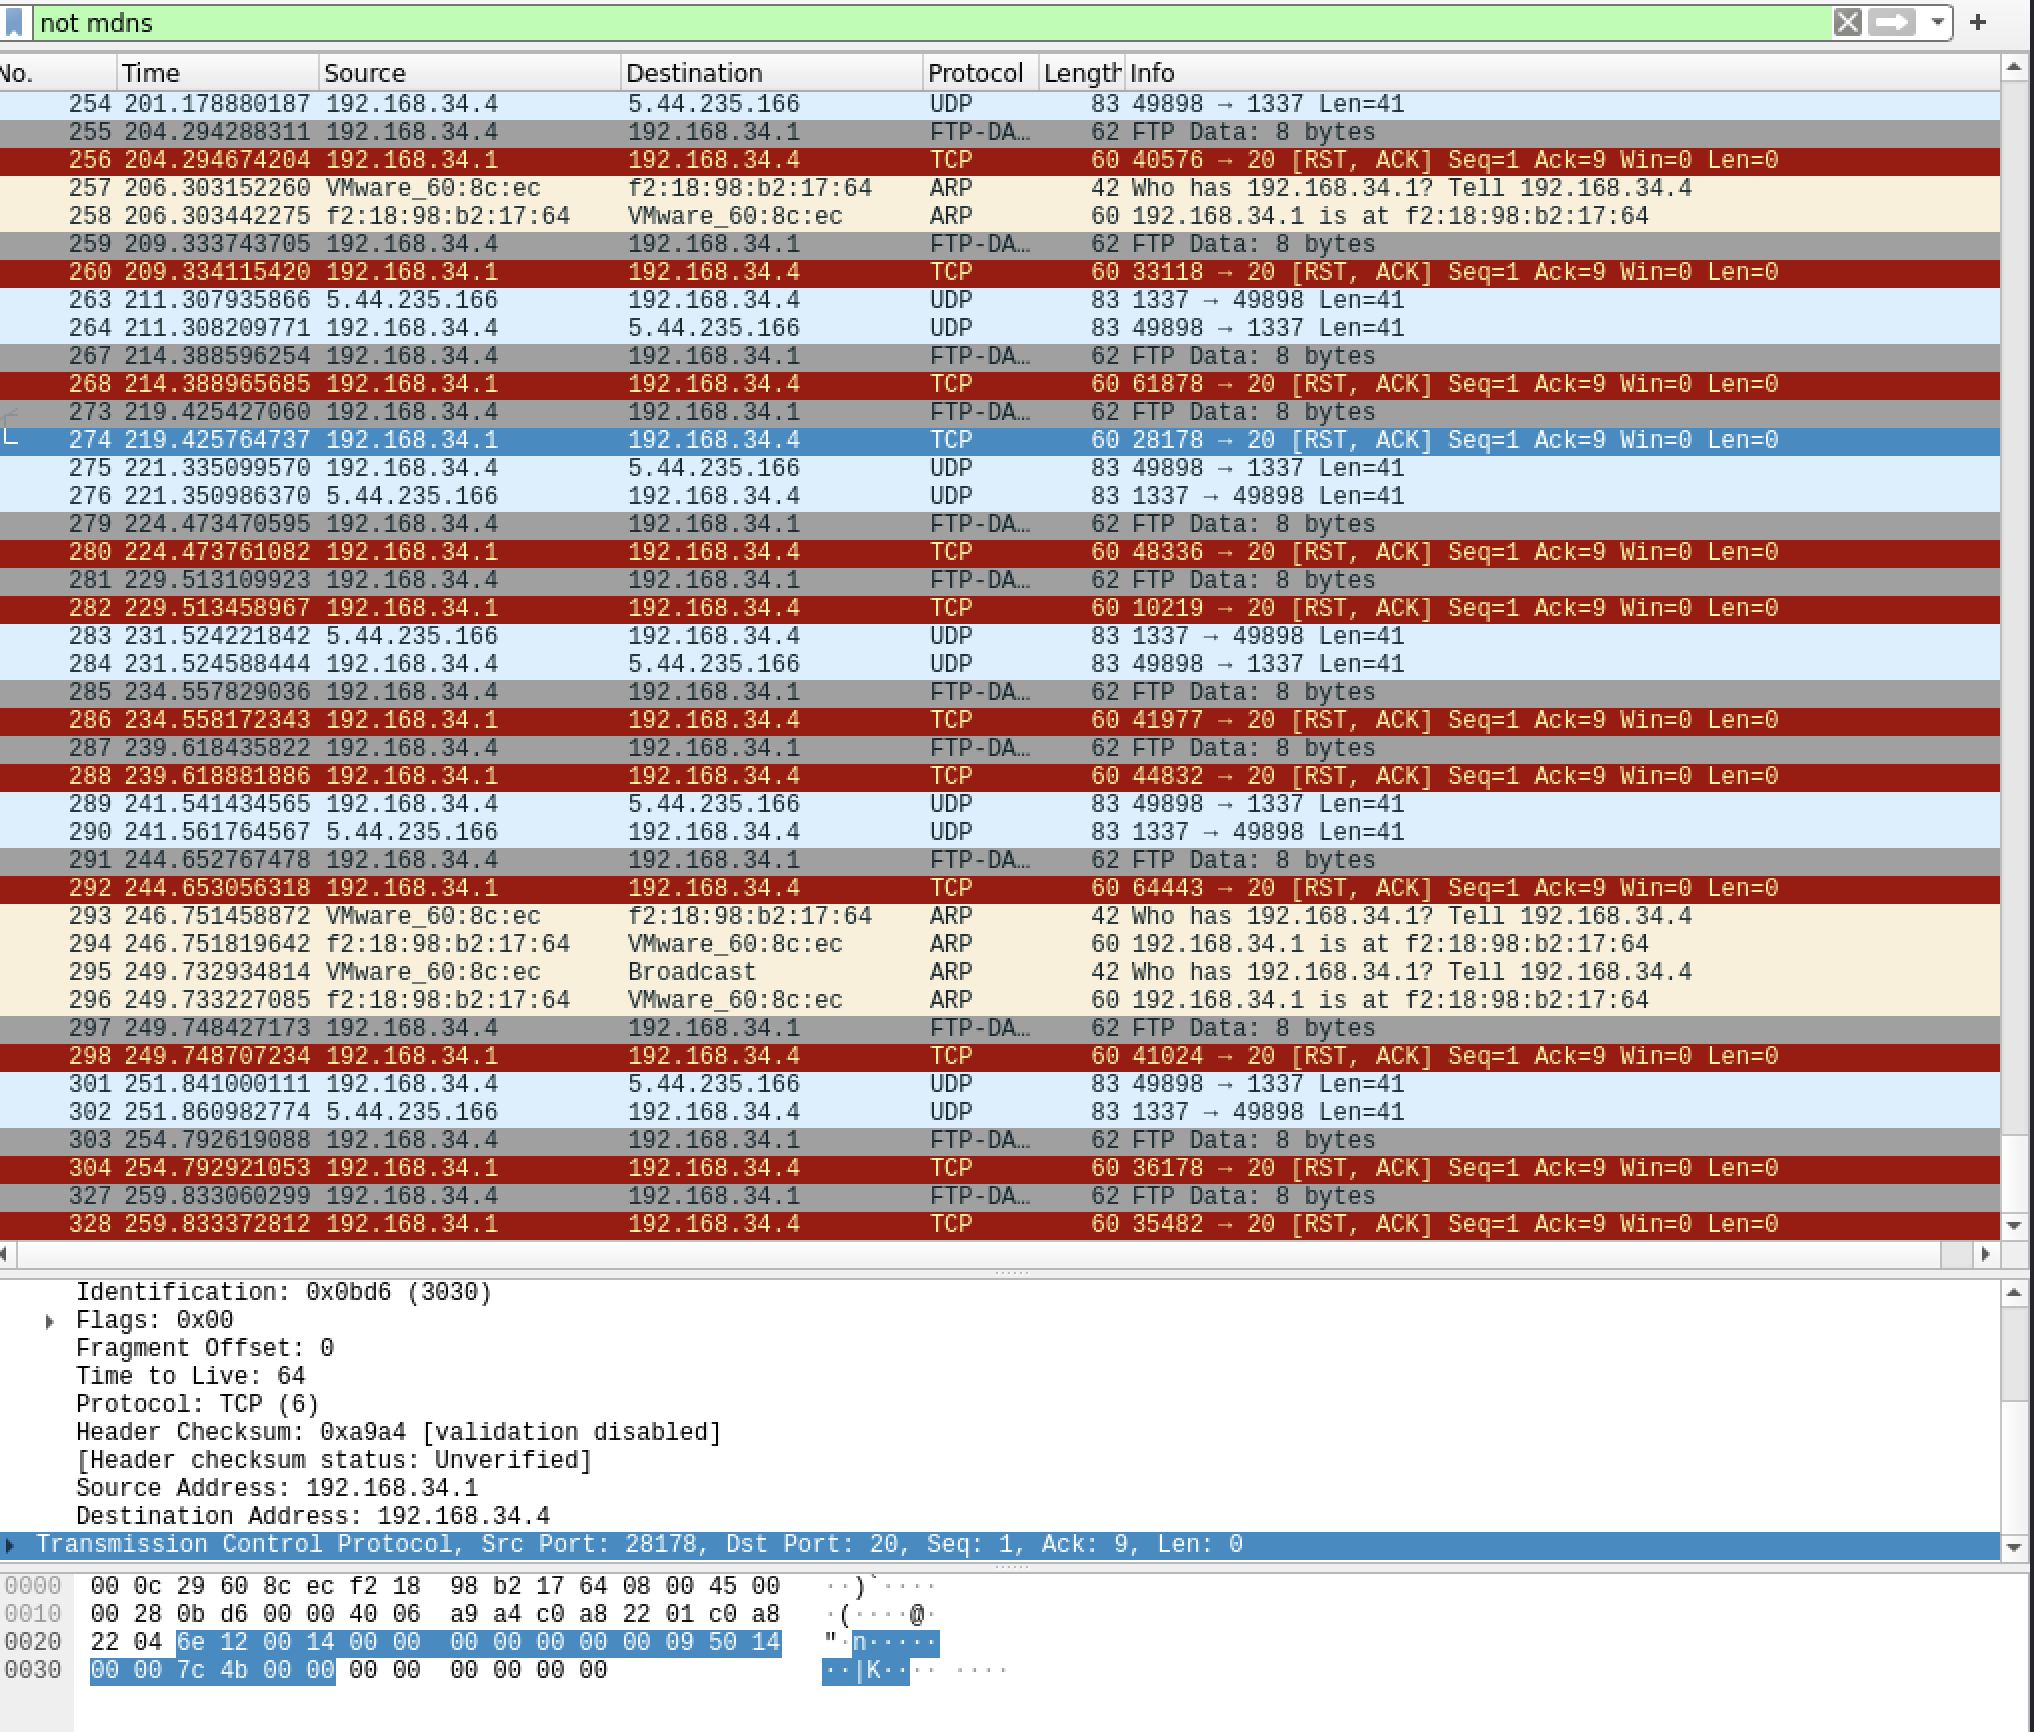
\includegraphics[scale=0.4]{wire3}
\caption{Paquets envoyés depuis wireshark}
\end{figure}

\section{Exercice 3}
\begin{itemize}
\item Ettercap est une suite complète pour les attaques Man in the middle. Elle propose le sniffinf de connexion, le filtrage du contenu à la volée et de nombreuses autres techniques. Elle prend aussi en charge la dissection active et passive de nombreux protocoles et comprend de nombreuses fonctionnalités pour l'analyse du réseau et de l'hôte.
\item L'ARP poisoning consiste à modifier l'association entre l'adresse IP (niveau 3) et l’adresse MAC, ou Ethernet (niveau 2) d'une machine cible. En effectuant ces modifications, il est possible de faire croire à une machine que l'adresse IP de son correspondant se trouve en fait à l'adresse Ethernet d'une machine pirate.
\end{itemize}
\begin{figure}[H]
\centering
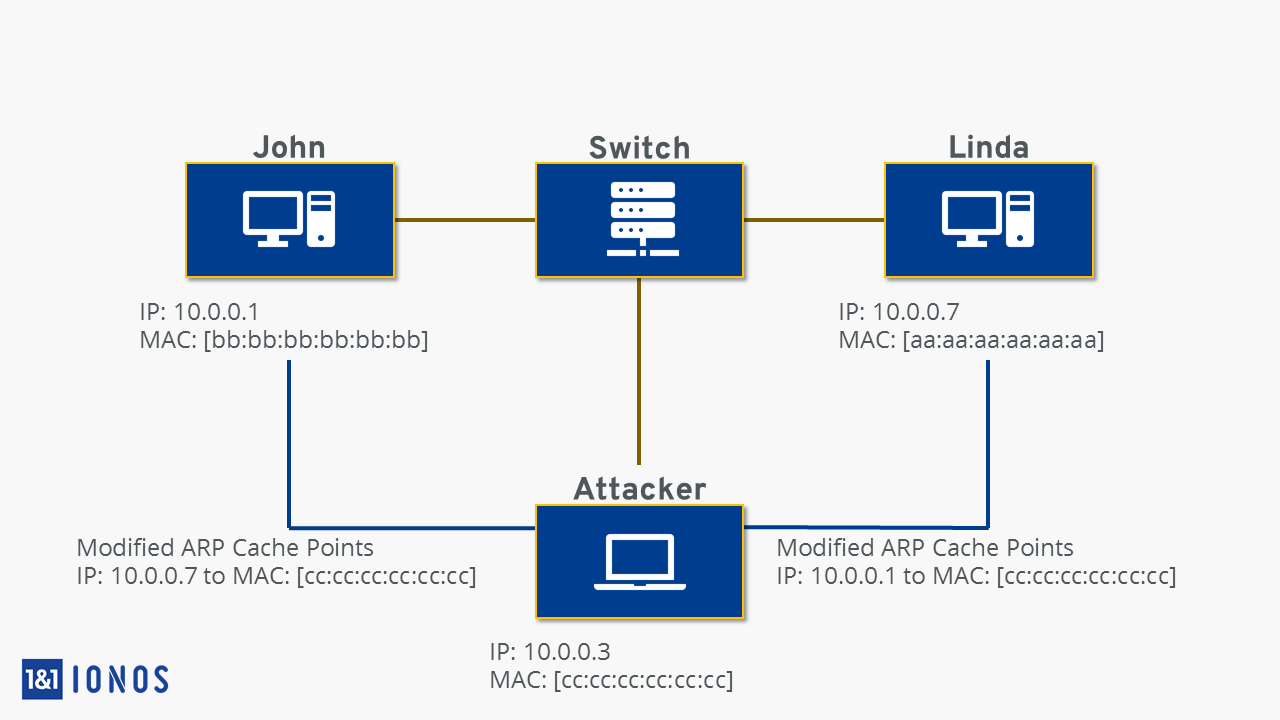
\includegraphics[scale=0.4]{arp_spoofing}
\caption{Paquets envoyés depuis wireshark}
\end{figure}
La commande arp -a sous unix permet de consulter la table ARP actuellement utilisée sur la machine. C'est elle qui va mapper les adresses IP rencontrées aux adresses MAC de chaque machine, afin de pouvoir les identifier au niveau de la couche réseau 2.
\begin{figure}[H]
\centering
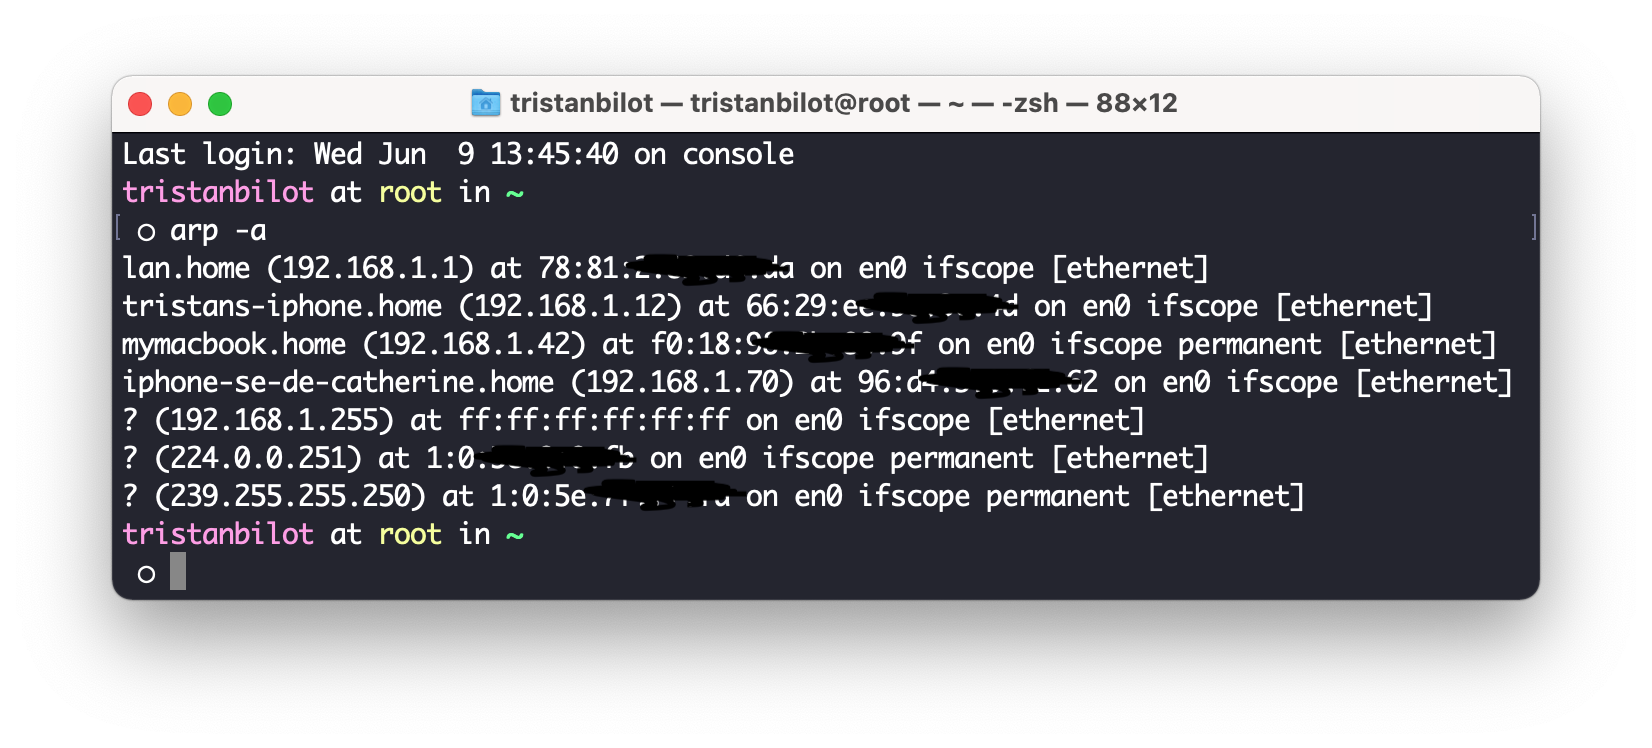
\includegraphics[scale=0.4]{arpa}
\caption{arp -a}
\end{figure}
\subsection{Attaque Man in the middle}
Afin de sniffer les connexions d'une cible sur un réseau, il faut l'adresse IP privée ce la machine à attaquer et l'IP de la gateway. Si une VM est utilisée, il faut bien penser à activer le mode bridge dans les paramètres de la VM afin qu'elle soit réellement connectée au réseau de la machine hôte.
\begin{figure}[H]
\centering
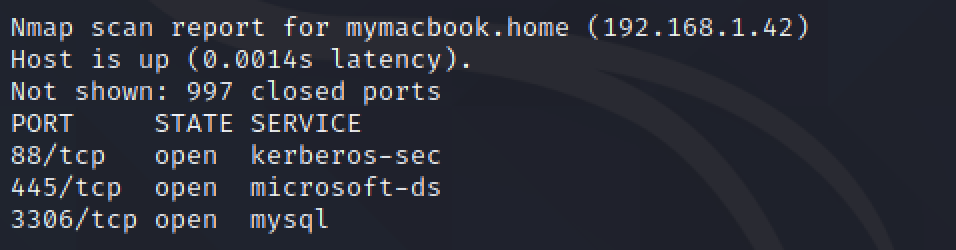
\includegraphics[scale=0.4]{target}
\caption{Récupération de l'adresse IP cible}
\end{figure}
\begin{figure}[H]
\centering
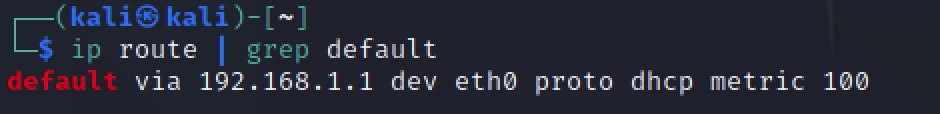
\includegraphics[scale=0.4]{gateway}
\caption{Récupération de l'adresse IP de la gateway}
\end{figure}
Avec ces deux adresses, il est possible de lancer l'attaque avec ettercap.
\begin{figure}[H]
\centering
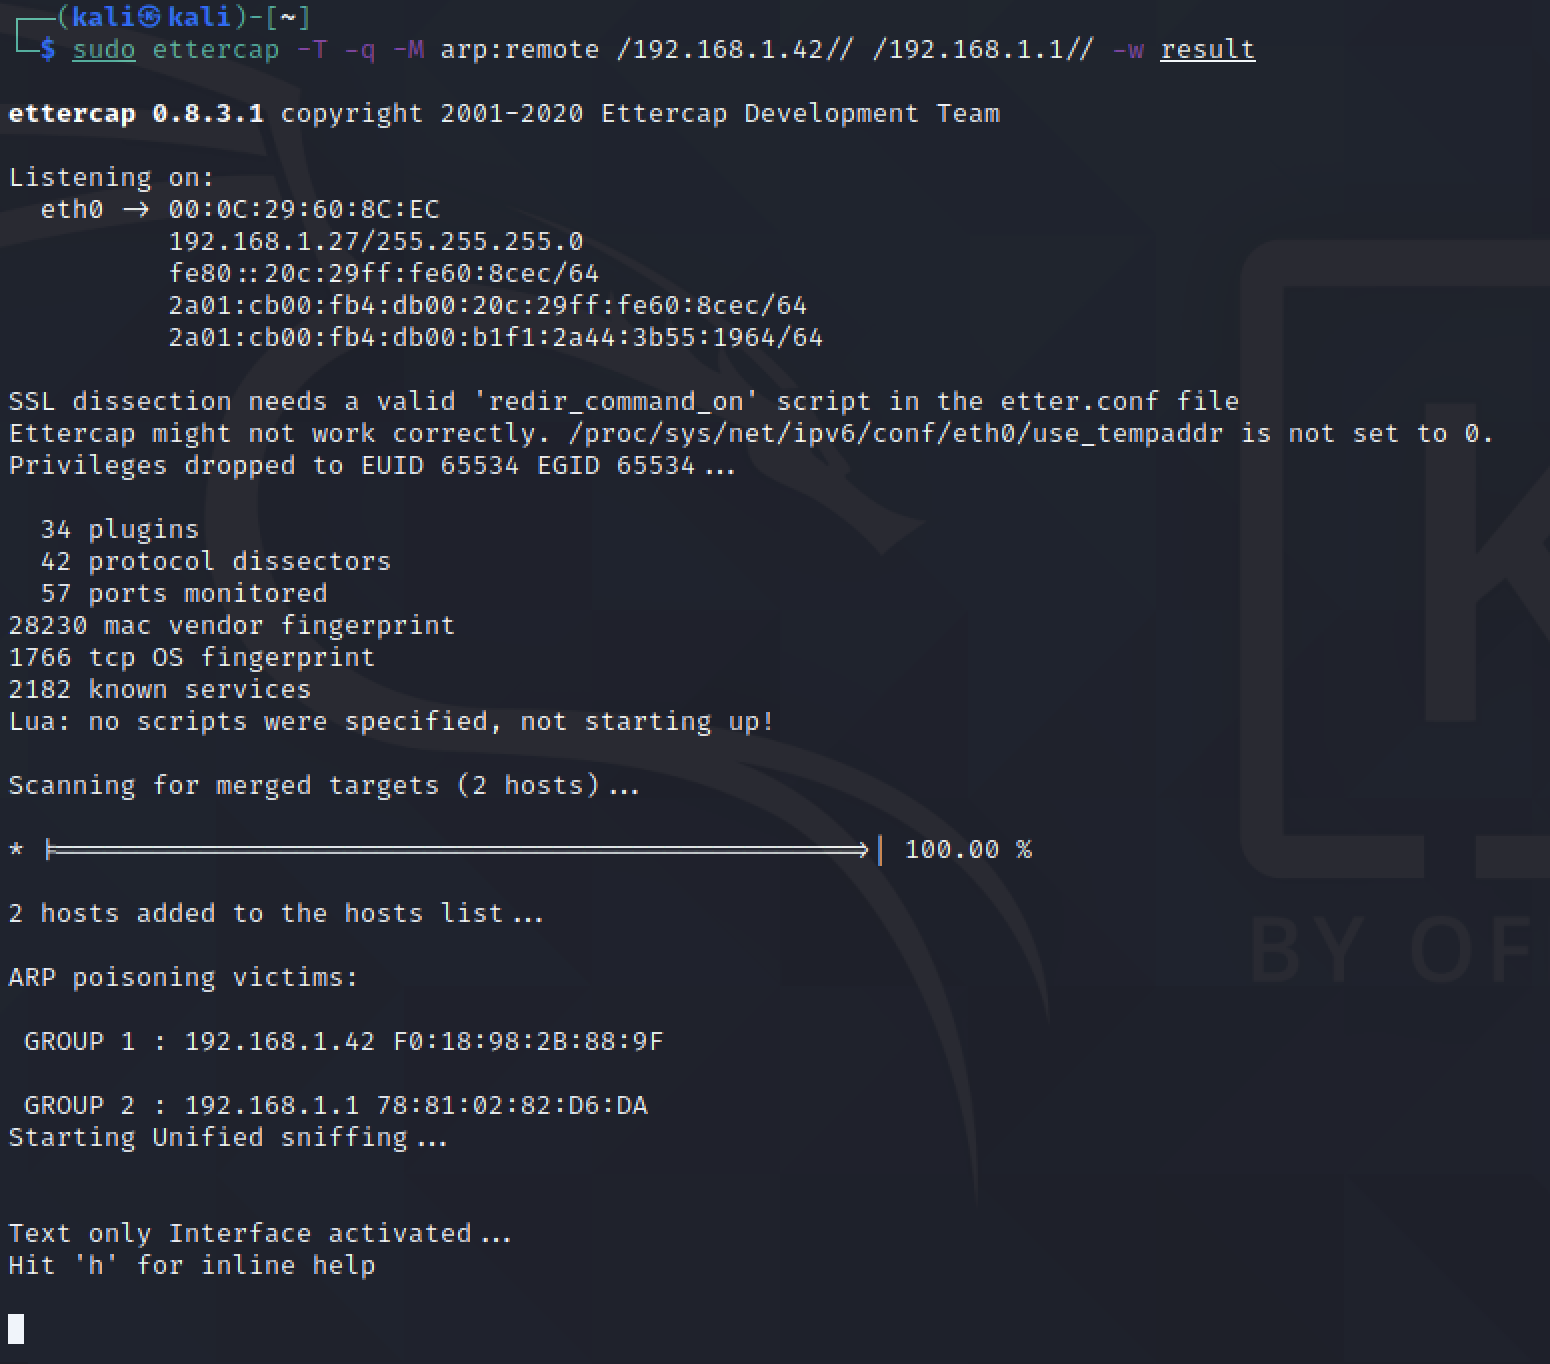
\includegraphics[scale=0.4]{ett1}
\caption{Attaque avec ettercap sur un MacBook du réseau local}
\end{figure}
Après quelques minutes de capture, il est possible de consulter le résultat du sniffing via wireshark avec le fichier result.
\begin{figure}[H]
\centering
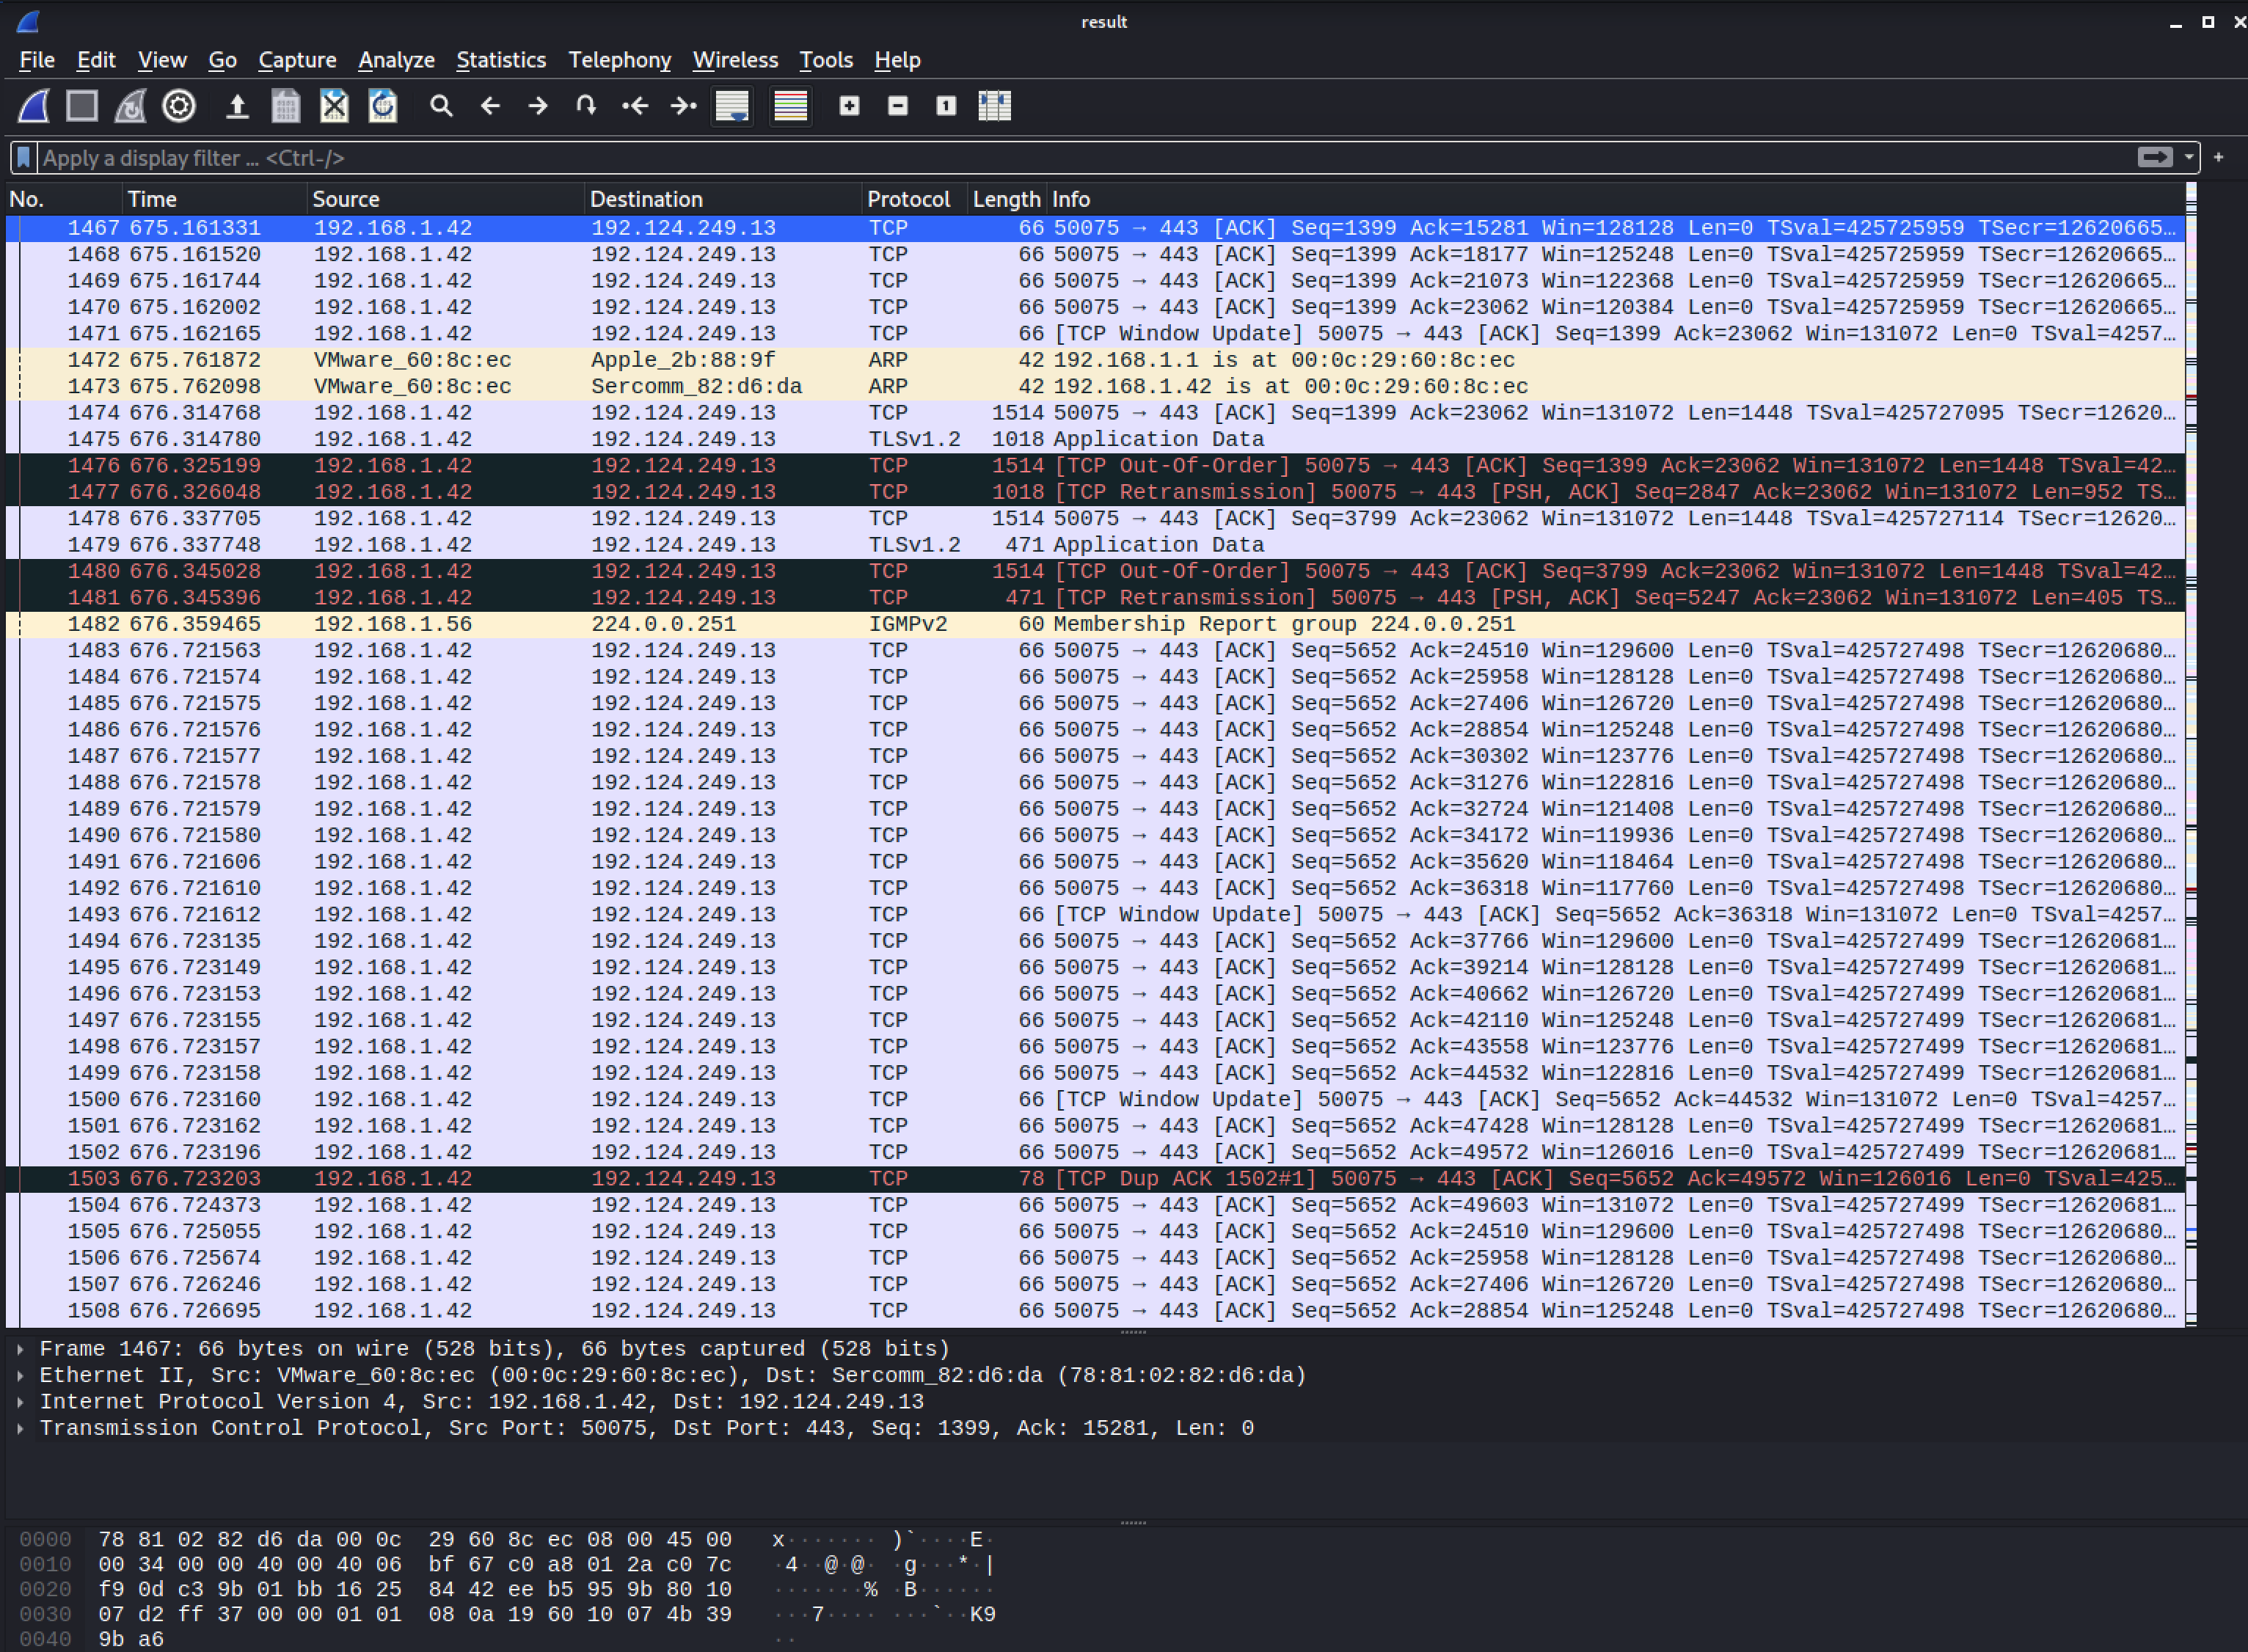
\includegraphics[scale=0.28]{wir2}
\caption{Record du réseau de la victime sur wireshark}
\end{figure}
Il est également possible de sniffer l'ensemble du réseau:
\begin{figure}[H]
\centering
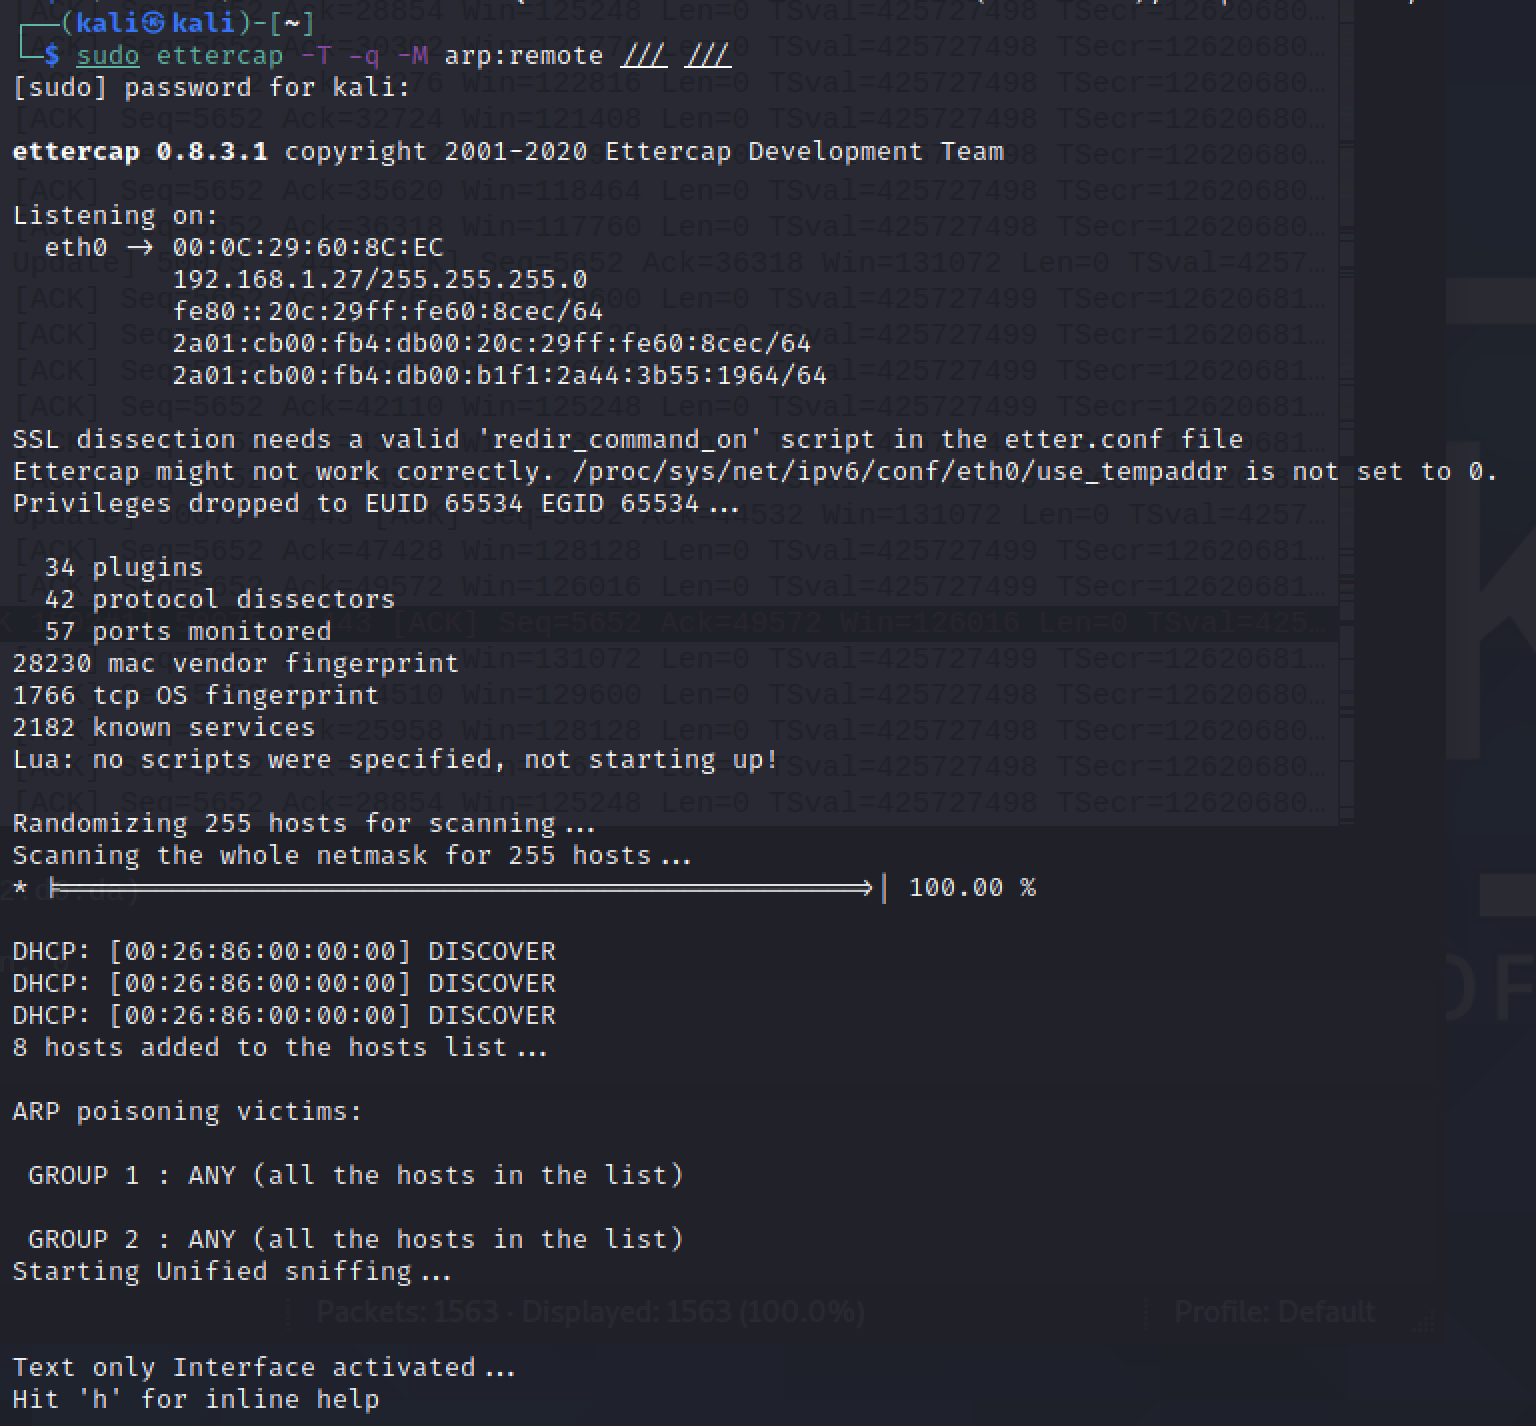
\includegraphics[scale=0.35]{full-net}
\caption{Sniffing du réseau en entier}
\end{figure}
\subsection{Etterfilter}
Etterfilter va permettre d'altérer ou de supprimer des paquets requétés par la victime. Il va être possible d'agir seulement sur les paquets transmis via http et non https car ils seront chiffrés et donc inaltérables.
Dans l'exemple suivant, il va s'agir de modifier les images de sites Internet requétés par une machine cible sur le réseau. Pour cela, il va falloir créer un script contenant la logique (le filter), puis compiler ce filter avec etterfilter pour l'utiliser avec ettercap.
\begin{figure}[H]
\centering
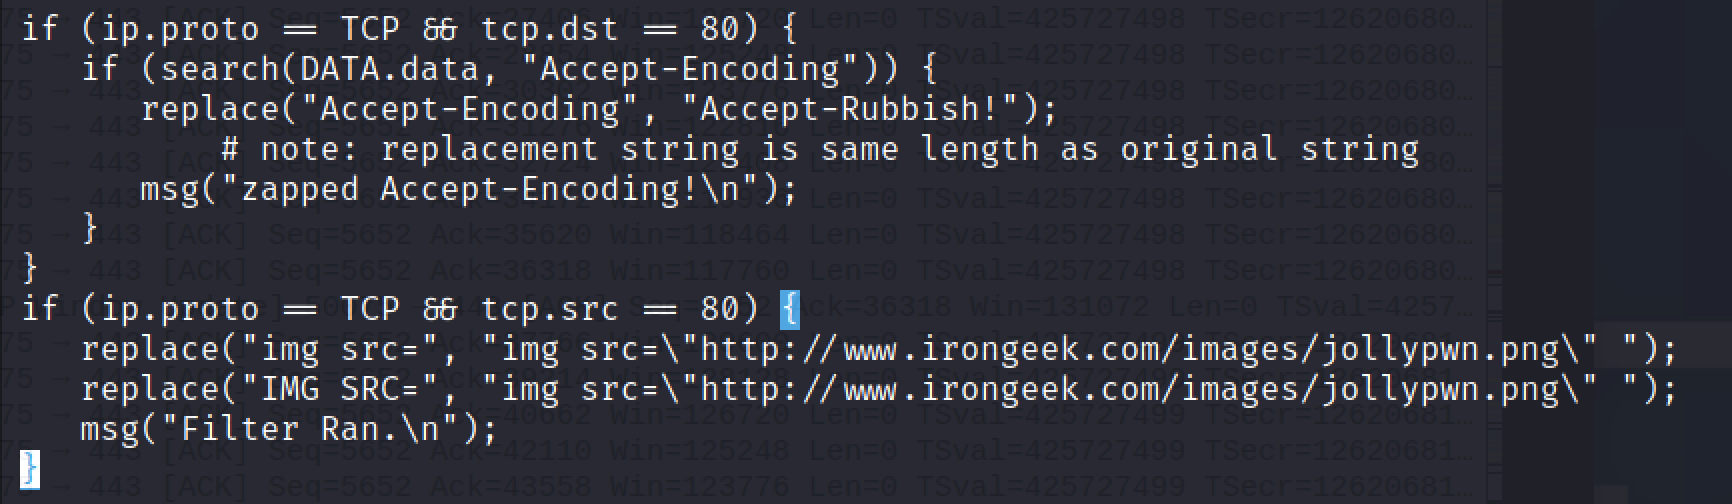
\includegraphics[scale=0.4]{filter}
\caption{Contenu du filter}
\end{figure}
\begin{figure}[H]
\centering
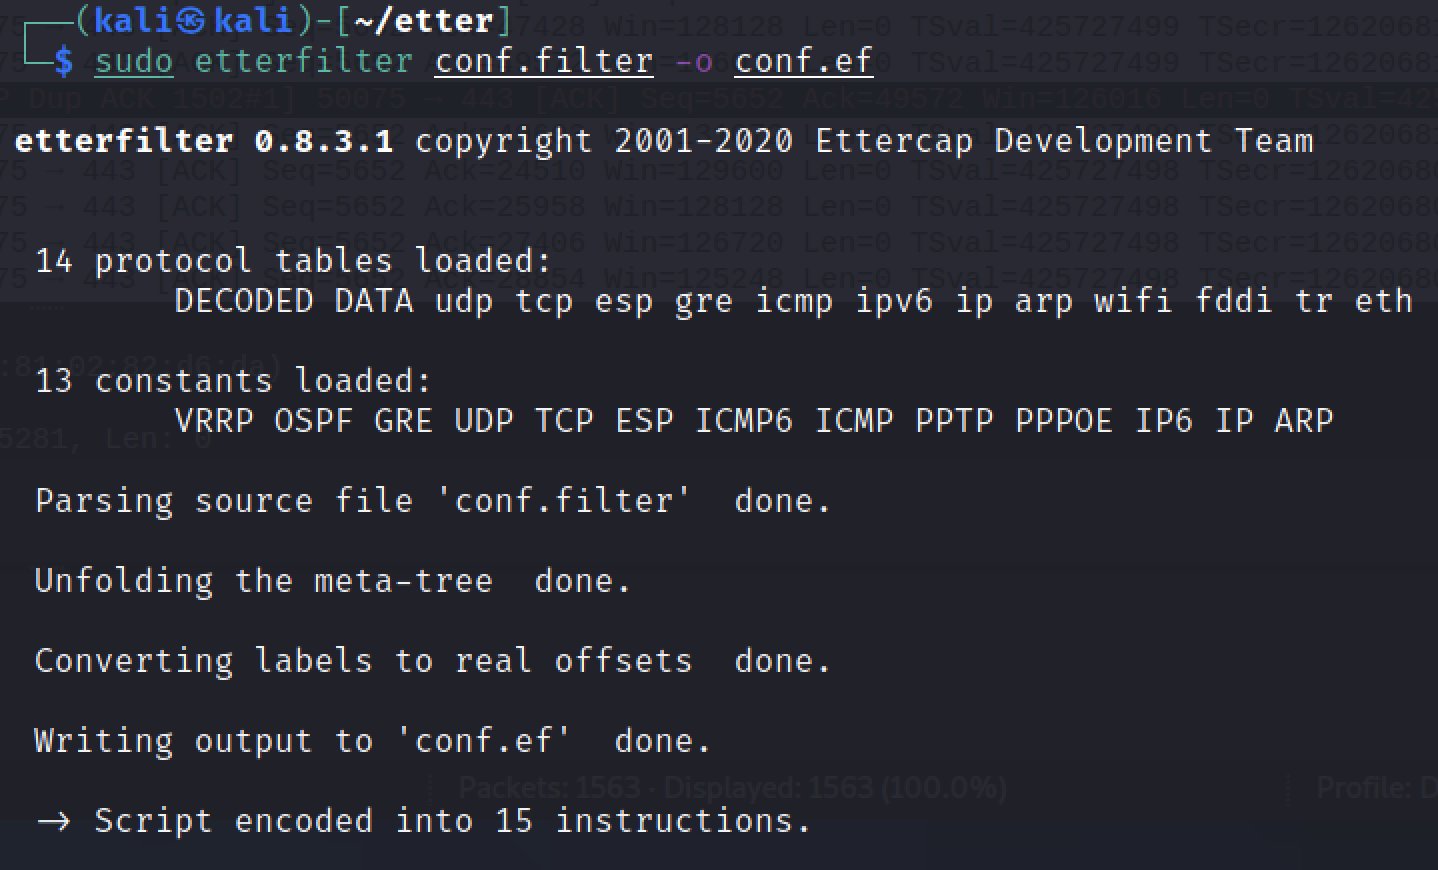
\includegraphics[scale=0.4]{compile}
\caption{Compilation du filter}
\end{figure}
\begin{figure}[H]
\centering
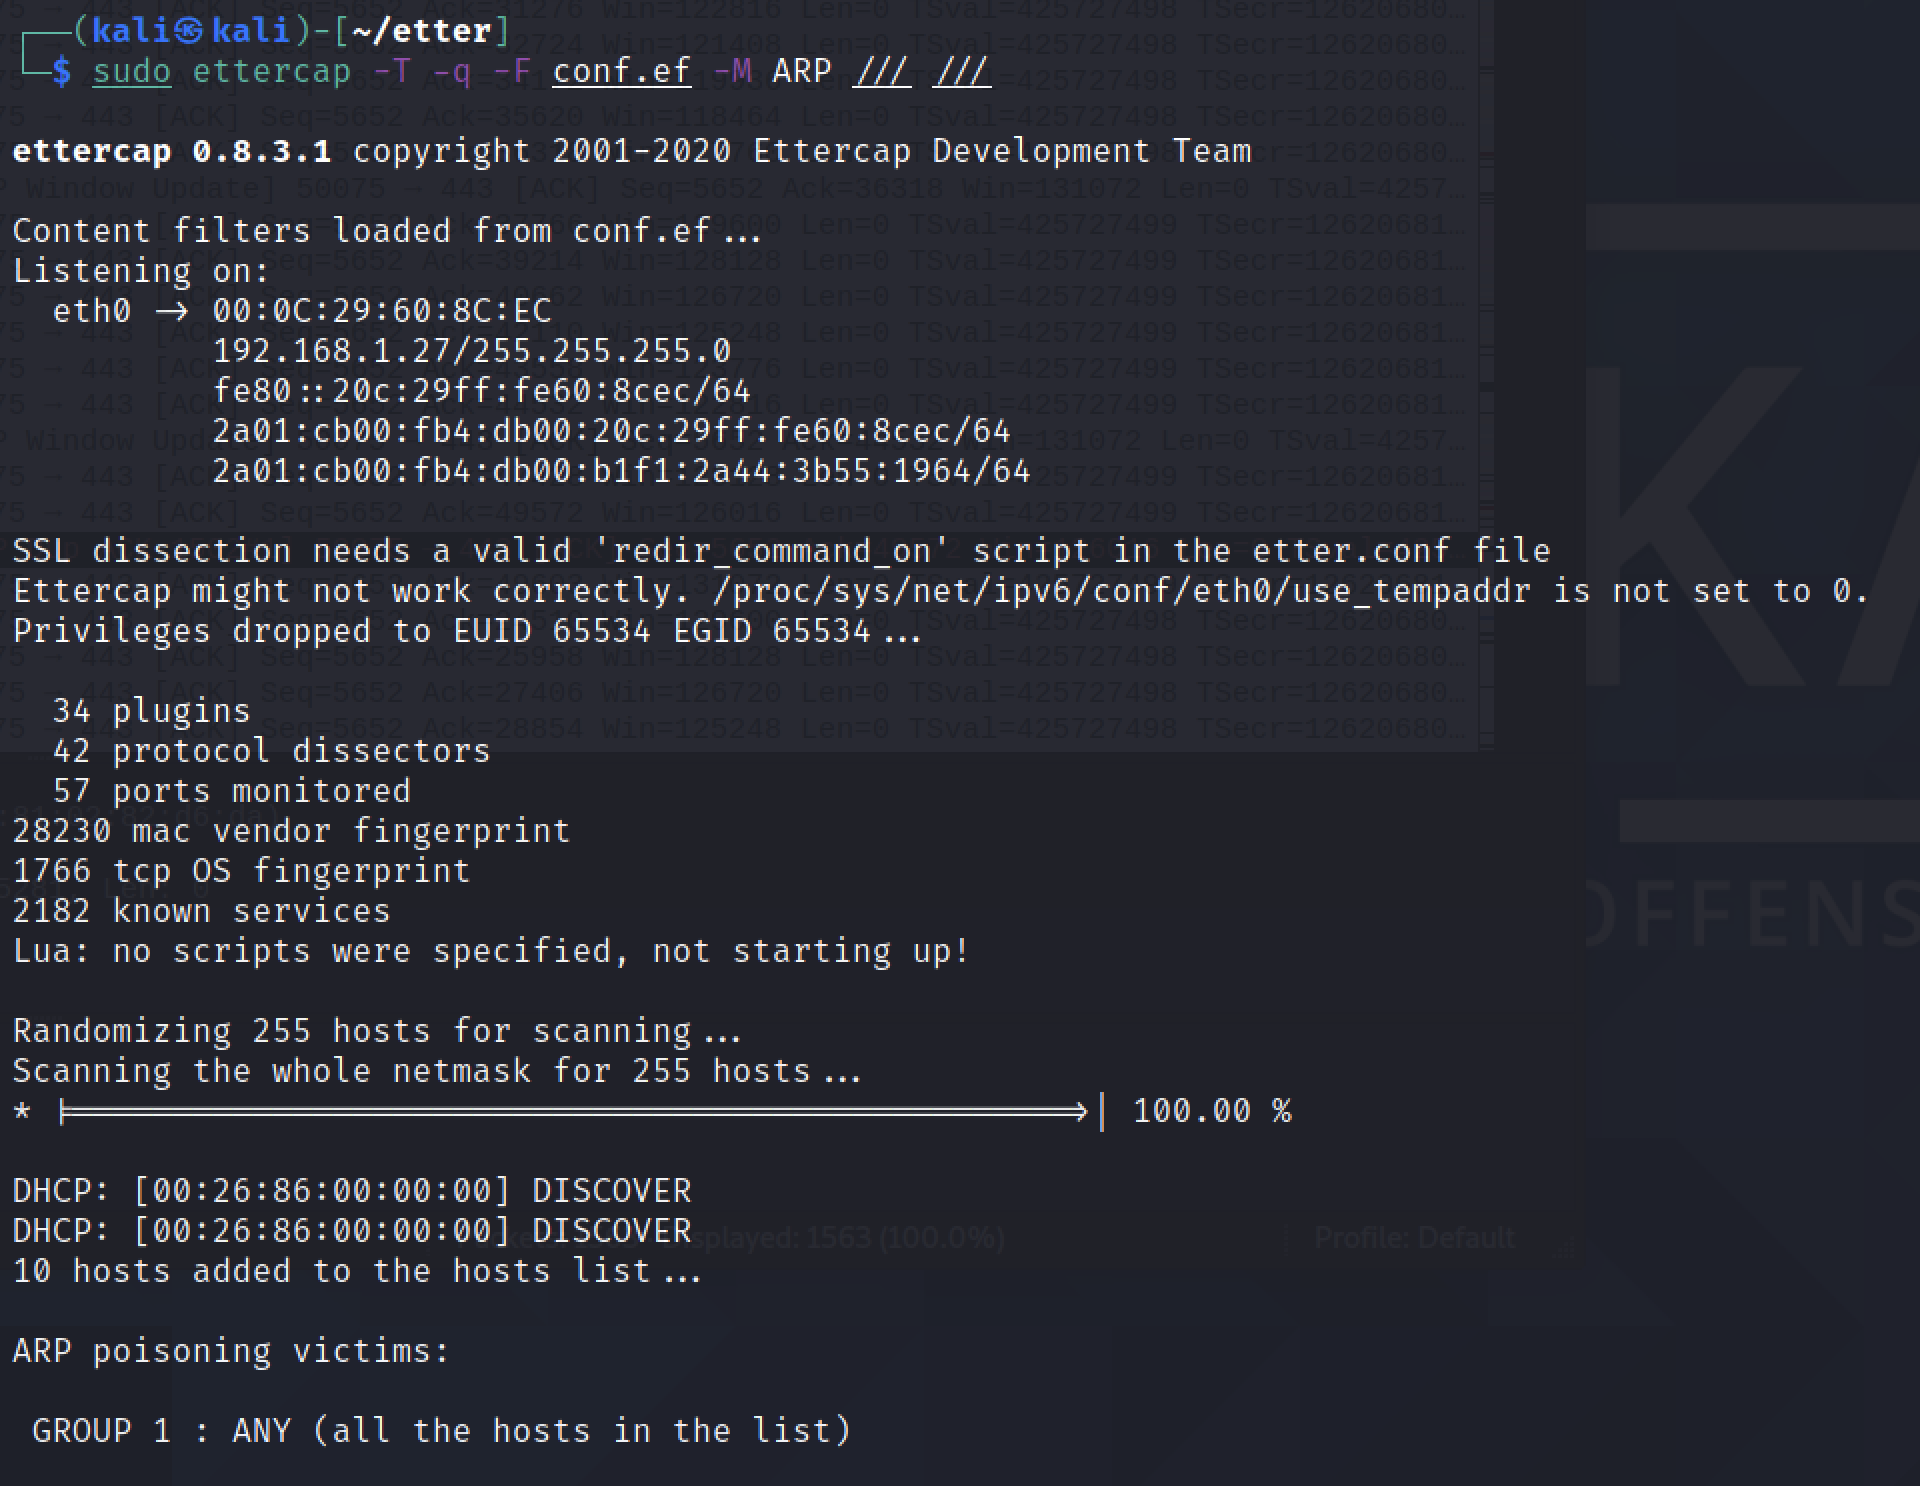
\includegraphics[scale=0.4]{cap}
\caption{Lancement du filtre avec ettercap}
\end{figure}
L'option -F permet de donner le fichier du filtre contenant les actions à effectuer sur le paquet et -M sp écifie s’il s’agit d’une attaque "man in the middle".\\
A présent, dès qu'un site http sera appelé sur la machine cible, les images utilisant la balise img seront remplacées par l'image ajoutée au filter.

\subsection{DNS poisoning}
L’empoisonnement du cache DNS (DNS Cache Poisoning) est une technique permettant de leurrer les serveurs DNS afin de leur faire croire qu’ils reçoivent une réponse valide à une requête qu’ils effectuent, alors qu’elle est frauduleuse.
Pour mener à bien une attaque par DNS Cache Poisoning, l’attaquant exploite une vulnérabilité du serveur DNS qui accepte alors des informations incorrectes. Si le serveur ne valide pas les informations reçues et qu’il ne vérifie pas qu’elles proviennent d’une source fiable, alors il stockera dans son cache ces informations erronées.  Il les transmettra par la suite aux utilisateurs qui effectuent la requête visée par l’attaque.
\begin{figure}[H]
\centering
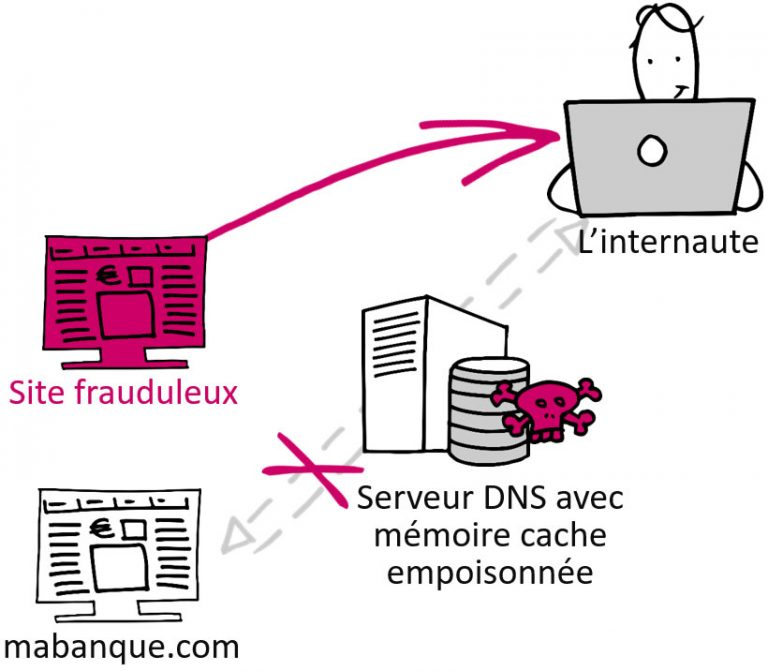
\includegraphics[scale=0.4]{dns-poisoning}
\caption{DNS poisoning}
\end{figure}
Tout d'abord, il faut ajouter la règle de redirection dans le fichier /etc/ettercap/etter.dns. Ici on ajoute la règle redirigeant www.myhostname.com à un site Internet personnel.
\begin{figure}[H]
\centering
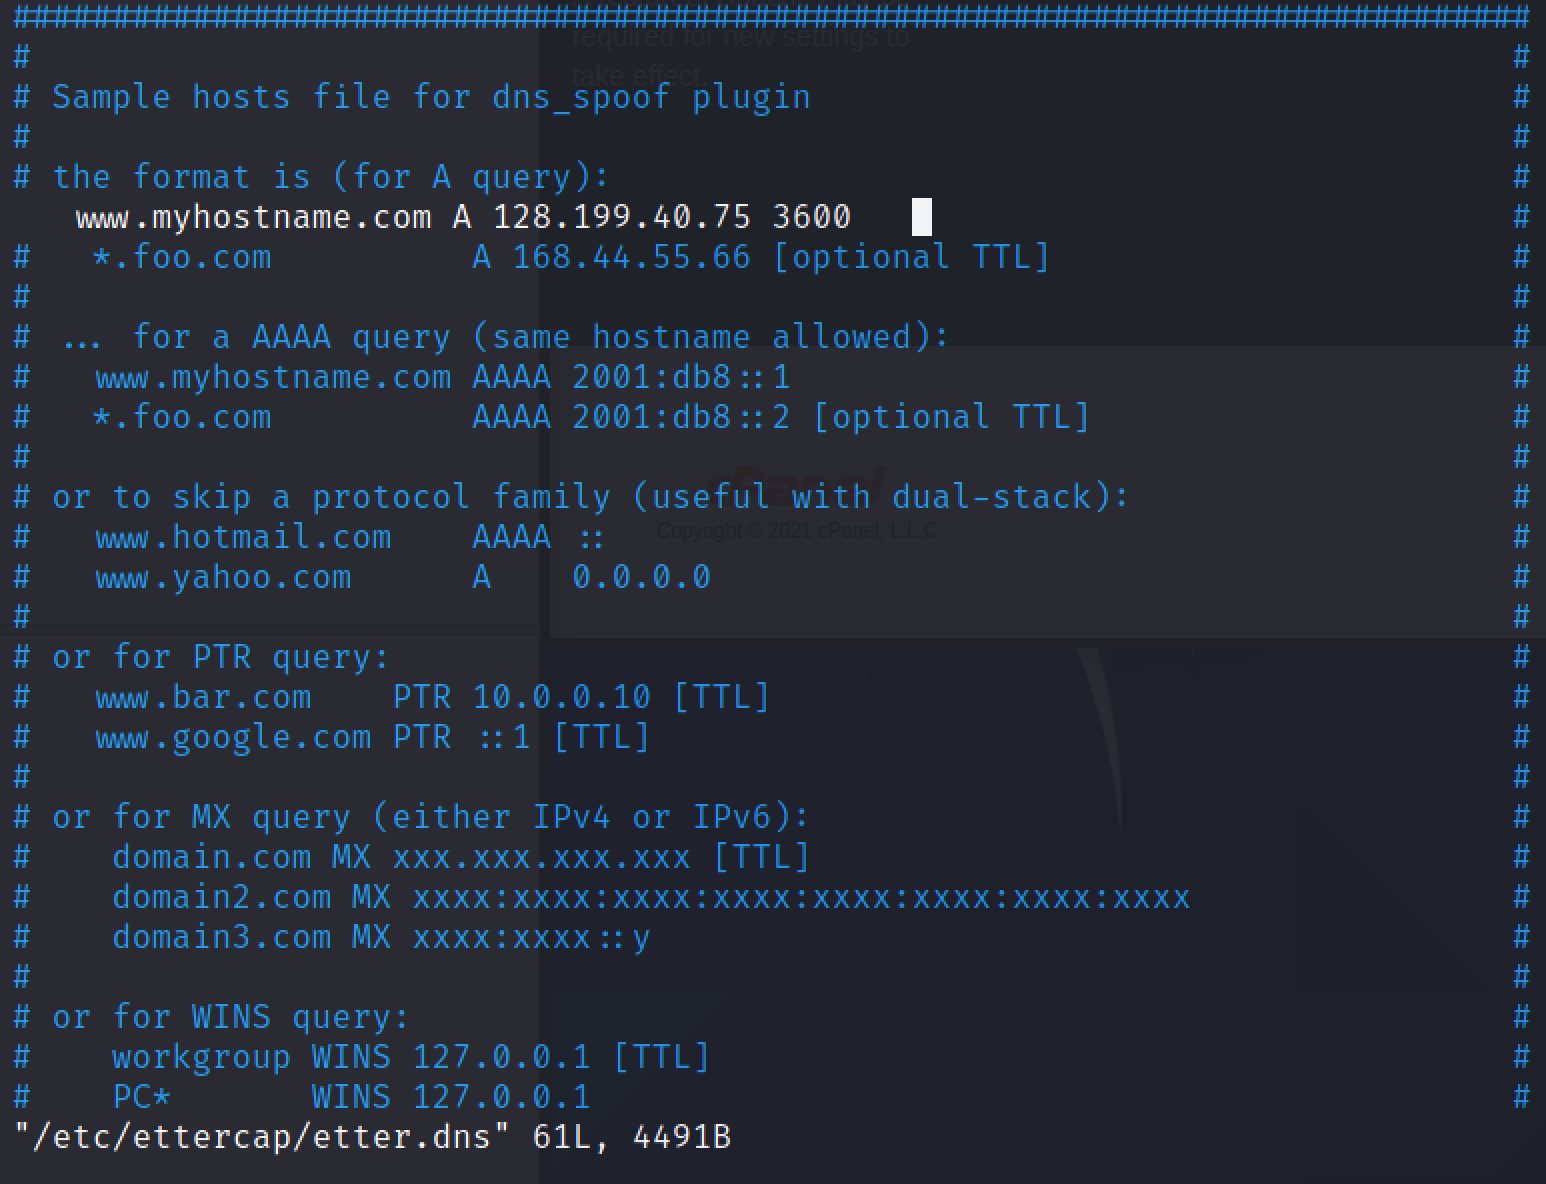
\includegraphics[scale=0.4]{redirect}
\caption{Redirection de www.myhostname.com à 128.199.40.75}
\end{figure}
Puis en lançant ettercap, toutes les machines du réseau seront redirigées vers 128.199.40.75 lorsqu'elles consulteront le site www.myhostname.com.
\begin{figure}[H]
\centering
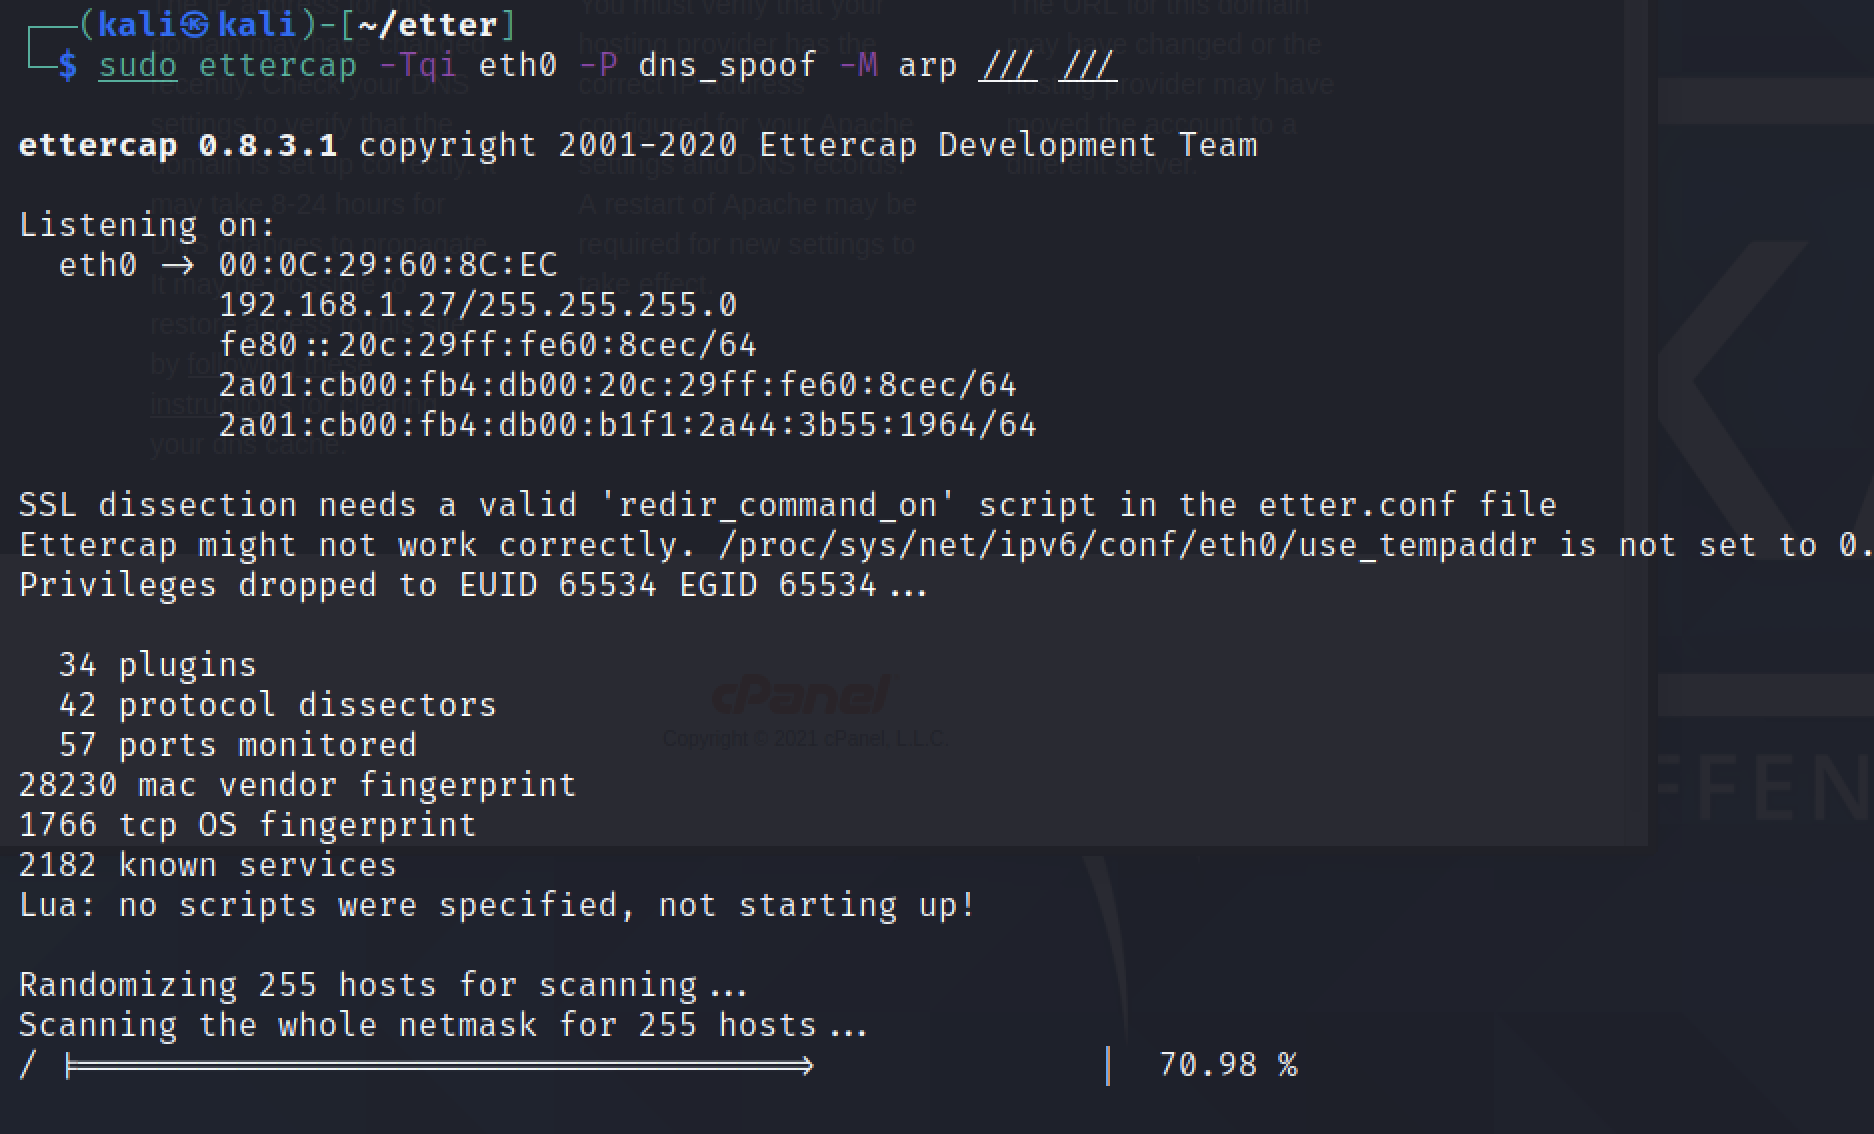
\includegraphics[scale=0.4]{dnsspoof}
\caption{ARP spoofing}
\end{figure}

\section{ARP poisoning: exemple concret (Arpspoof)}
L'outil python Arpspoof a permis de créer un scénario concret d'ARP poisoning, c'est à dire de modifier la table ARP d'une machine distante sur un réseau afin que le passerelle devienne l'attaquant. Dans un premier temps, le contenu original de la table ARP a été stockée dans un fichier "before" puis l'ARP spoofing a été lancé côté attaquant et enfin la table ARP a été de nouveau sauvegardée mais cette fois-ci dans un fichier "after". On aperçoit que l'adresse MAC de la gateway a été modifiée par l'adresse MAC de l'attaquant. L'attaque est un succès. 
\begin{figure}[H]
\centering
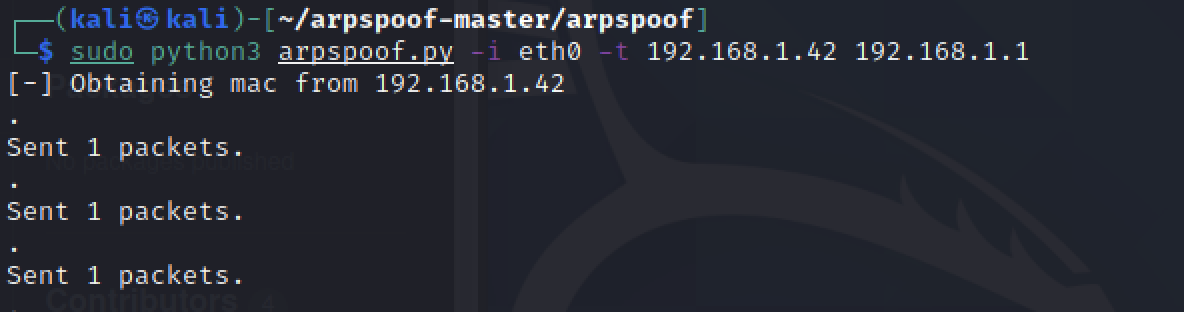
\includegraphics[scale=0.4]{arpspoof2}
\caption{Lancement de l'attaque d'ARP spoofing}
\end{figure}
\begin{figure}[H]
\centering
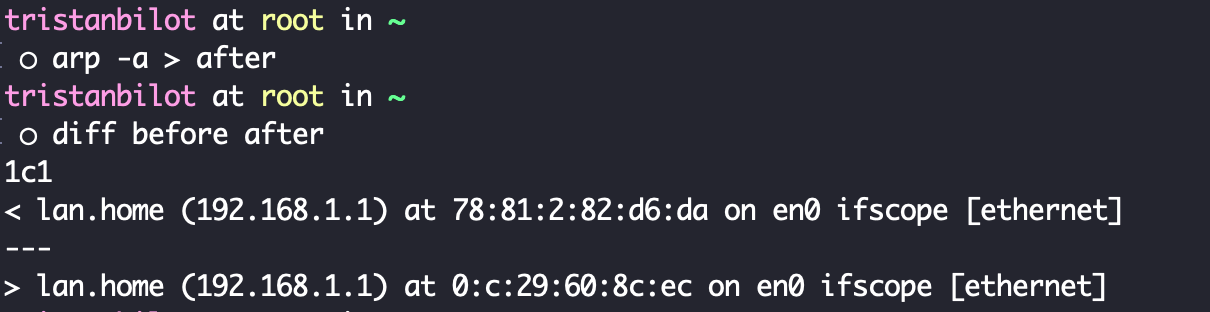
\includegraphics[scale=0.4]{arpspoof}
\caption{Comparaison de la table ARP de la victime avant et après l'attaque}
\end{figure}

\section{ARP spoofing implementation avec Scapy}
Afin de comprendre de façon claire le fonctionnement de l'ARP spoofing, voici une implémentation de l'attaque avec Scapy. Afin de rétablir l'état initial de la table ARP de la victime et de la gateway, il suffira de faire un ctrl+C.
\begin{figure}[H]
\centering
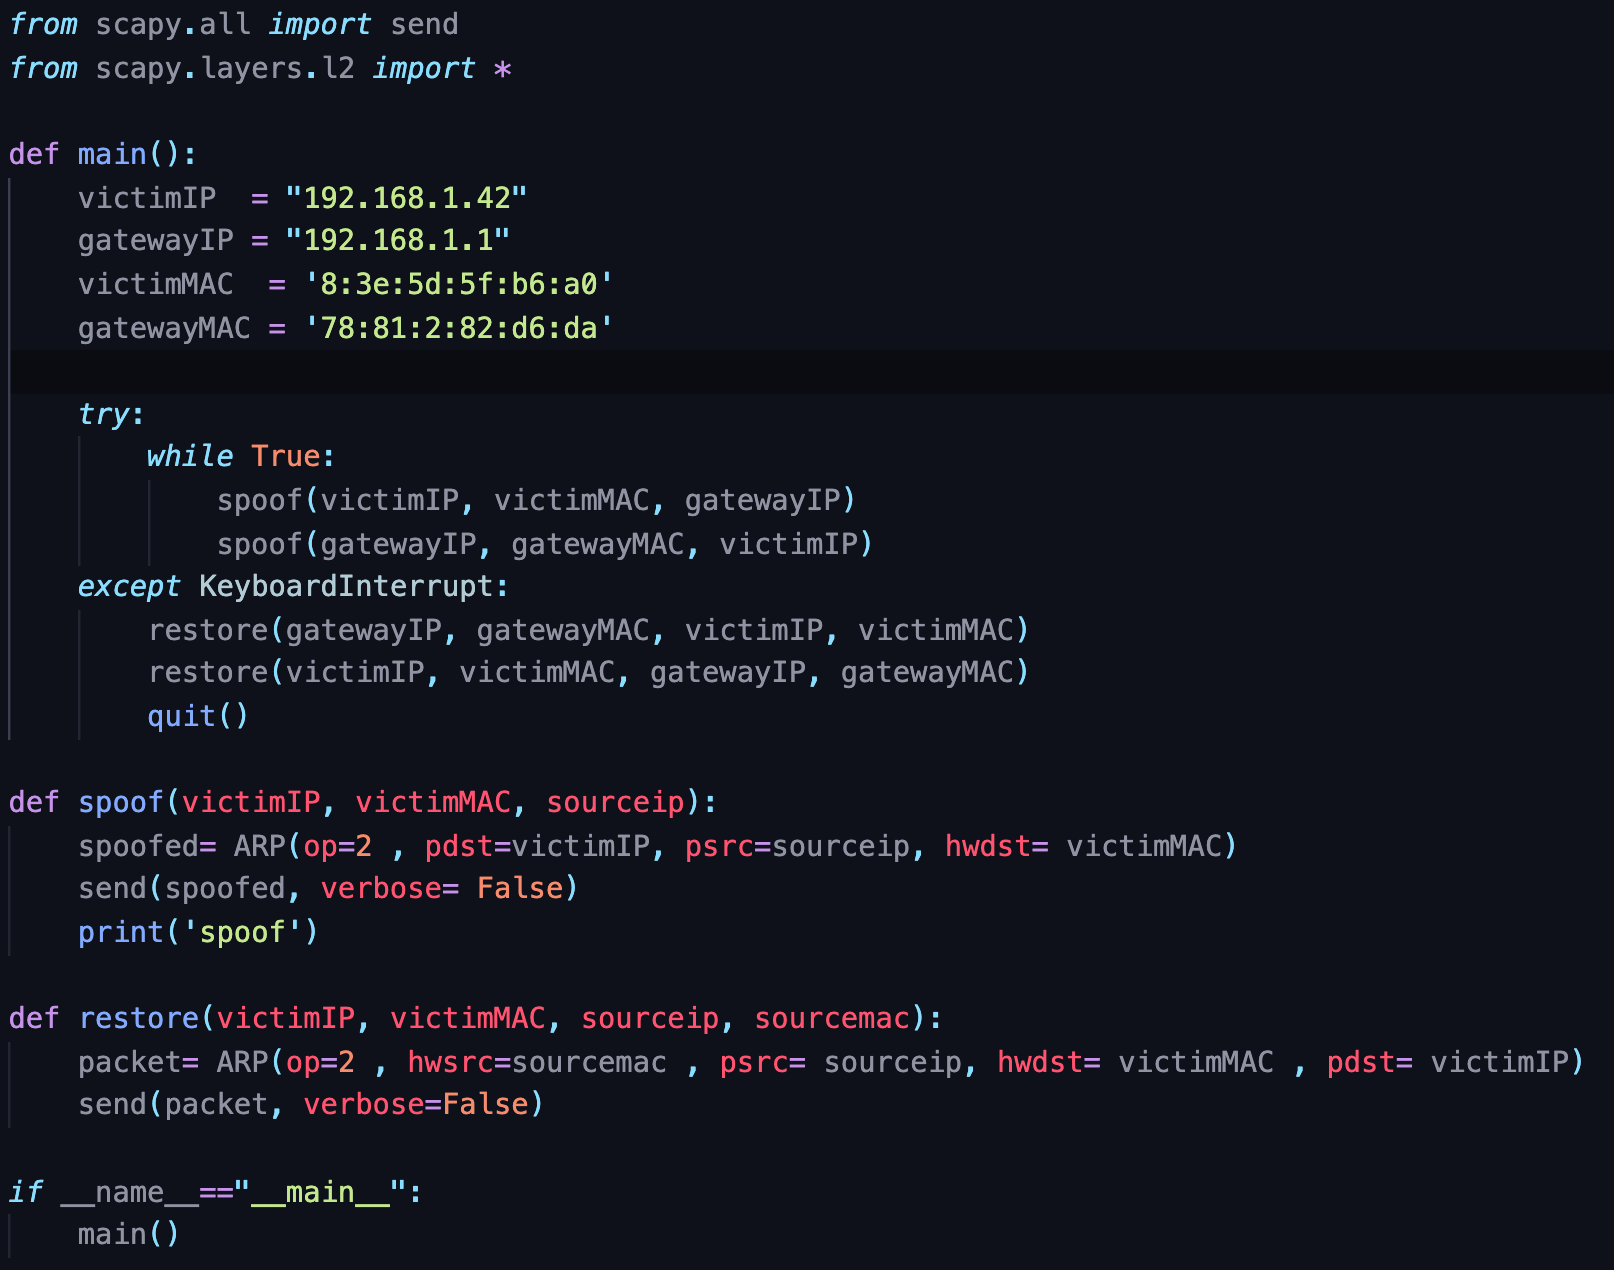
\includegraphics[scale=0.4]{myspoofcode}
\caption{Code de l'ARP spoofing}
\end{figure}
\begin{figure}[H]
\centering
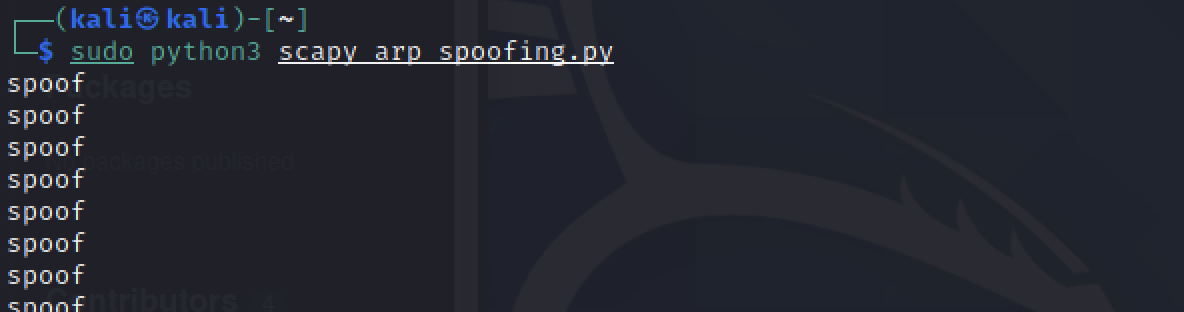
\includegraphics[scale=0.7]{myspoof}
\caption{Lancement de l'attaque}
\end{figure}
\begin{figure}[H]
\centering
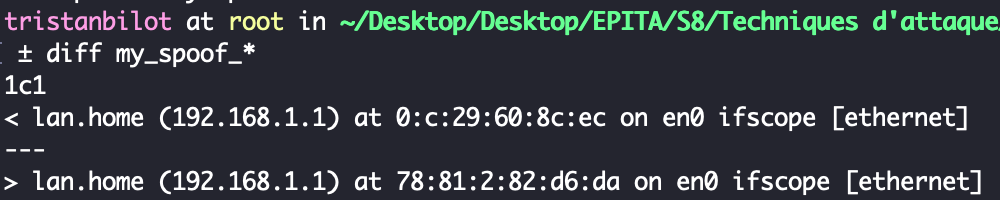
\includegraphics[scale=0.7]{myspoof2}
\caption{Table ARP altérée de la victime}
\end{figure}


\end{document} 

